\documentclass[11pt,a4paper]{article}
\usepackage[T1]{fontenc}
\usepackage{indentfirst}
\usepackage{section}
\usepackage{graphicx}
\usepackage{physics}
\usepackage{scalerel,amssymb}
                                                                                                  
\graphicspath{ {./} }


\title{Why Should We Use Reimannian Manifolds in Physics?}
\date{\today}
\author{Son Hoai An}

\begin{document}
	\maketitle
	
	\tableofcontents
	\pagebreak
	
	\section{Introduction}
	As  we are leaving in three dimentional space, our motions or any objects can be describle in the coordinate of three direction or in three degree of  freedom.  For example, we can describle and object as a cube in our living space as connections of some lines with the set of three direction collections as left-right, up - down, forward - backward (this will need some imaginary in spartial geometry), however, we can not express full features of curve space as how deep, and curved is it.  That seemed to be a major problem for both mathematicians and physiscs to explain phenomena of gravitation, the bending of light by heavy massive objects, black holes, gravitational waves, etc.  Understand this limitation of  three dimentional space, Einstein constructed and built his own space theory which has more strong and essential tools to indicate events, properties of space-time based on Riemannian space.
	
	On 27th , January 1921, Albert Einstein gave his address on  the topic Geometry and Experience  to introduce his geometry  -  an inital part in Einstein's General Theory - which has strong and solid connection with Riemannian geometry and space. Since this, our view of space and time was changed and Riemann space places a crusial role reflect the impact of physical phonomena, such as gravitational attraction of large objects exert on smaller one and on the fabric of space and time. 
	
	\section{Historical Development}
	\subsection{Non-Euclidean Geometry}
	In Euclid's space, we have five basics postulates as:
	\begin{itemize}
		\setlength{\itemindent}{.2in}
		\item  There is one unique straight line joinning any two distinct points.
		\item Every straight lines can be spread  endlessly.
		\item  It is possible to draw a circle with any given a center point and radius. 
		\item All right angles are equal to each other.
		\item  A given line \textit{m} and a point \textit{P}  not on  \textit{m}  alway have exactly one  line \textit{n} passing through \textit{P} and parallel to \textit{m} .
	\end{itemize}
	
	In narrow way, we could understand parallel means "lines do not cross or intersect each others". Therefore, the fifth could fail in two different cases. One is for a very large curve and there is no straght line through \textit{P}. Another is a hyperpola lines passing through \textit{P} and does not cross \textit{m}.
	 However, such a long time, people believed that there is no cases or posible for the fitth to be false in the space region  due to two reasons. The first was that God does things carefully and not have any faults - the space eternally has one form. The second, a flatness of space based on Immanuel Kant, the German philosopher - space is as large as our own imaginary minds, we can not have any space unsastify Euclidean's postulates. In his statement, we could understand the term of "a creation of our own minds"  that means we can not see or imagine seeing nany thing that is not located in considerable space.  
	 With beliefs in God, we could not dissagree in this age, however, for Kant's argumentation, we can  prove that the non-Euclidean spaces exist naturely by using  a space as the  surface of spheres in 3-dimentional space because there is no straight line in this space (all lines are curves in it's local or global positions). 
	 
	 \begin{center}
	 	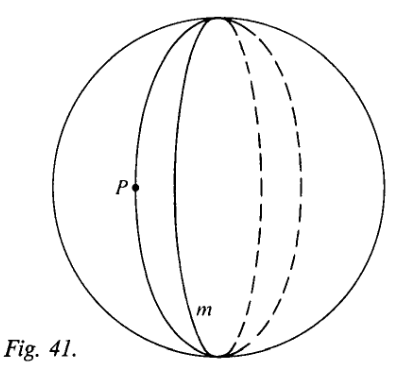
\includegraphics[scale=0.35,alt={the sphere with lines connecting two poles}]{./Fig41_sphere.png}
	 \end{center}
	 
	 
	 So, the parallel postulate of Euclidean space failed to protect itself as well as Kant's argument, Furthurmore, in sphere space, we can see infinite circles connecting or joining two polar points - it  violates the first postulate. 
	 These reasons lead to two new models of space called curved-space model and  field model - a flat space and curved line; the dual views of space is essntial to Einstien's General Theory of Relative  in which gravitational fields are defined in term of the curvature of space-time.
	 
	 \subsection{Curved Space}
	 There is a hard question for us to demonstrate our space as  a sphere-like object. We can not deny that our world (or our Earth) always describles in the 3-dimention space, and  to simulate it in a material world, we shoud place it in an extra dimention to show or illustrate how it moves or travels from a place to somewhere else, and measure it's actions in periods of time. The dimetion for that work we call the fourth dimention but we can not recognize and contact in real life. The statement above points that if we have "straight lines" in sphere surfaces, where we are living,  they will be actually  and truly curved  when our space is moving along this unknown direction. 
	 
	 Many scientists used to believe that our space was a spherical 3-dimention space. Despite not completely believing in this idea, Einstein still put it forward because it showed a view of  an finite space without boundaries, supported for the idea of  a space that expands continuously, includes infinitely  many stars, many planets,  many civilizations.
	 
	 From now on, we contruct pictures of  a point in an "flat space" and in a "curved space"
	 
	 \begin{center}
	  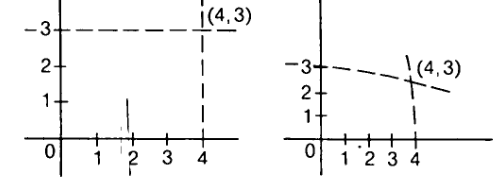
\includegraphics[scale=0.75]{./Fig66_coordinate.png}
	 \end{center}
	 This picture shows us how both Euclidean space and curved space present their element. From this picture, we can see the region which are made by the line $y = 3$ and  $x = 4$  look like different in two coordinate, this cam be explain by the the curved degree of coordinates. If the space is curved more and more, the region must be smaller and smaller as it should be when it projected to the flat coordinate. To reserve the distance when moving from one coordinate type to others, we need  transfromations, which take huge effort to find, to conform object's shapes. From this point, mathematicans introduced a new advanced tool so that we can use to transform from one co-ordinate to other one - called tensor - in the form of a matrix with its elements are a function of the coordinate axises. In two dimentional space, we have a function $G(x,y)$  from a distance $ds^2$ as	 
	 \begin{center}
	 	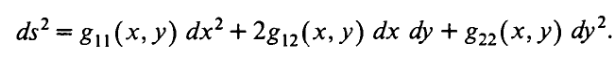
\includegraphics[scale=0.4]{./ds2d.png}
	 \end{center}	 
	the g-function is 	
	\begin{center}
		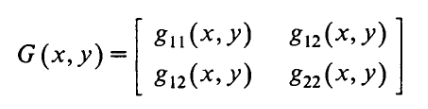
\includegraphics[scale=0.4]{./G2d.png}
	\end{center}
	For three dementional space, we have a similar equation for $ds^2$  
	\begin{center}
		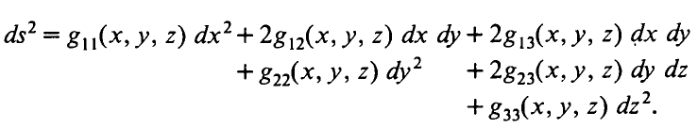
\includegraphics[scale=0.4]{./ds23d.png}
	\end{center}	 
	and g-function should be
	\begin{center}
	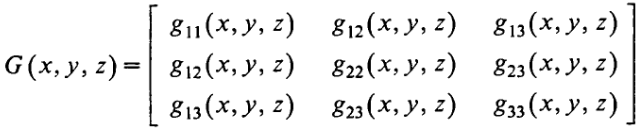
\includegraphics[scale=0.35]{./G3d.png}
	\end{center}
	The function G is called the metric tensor. It lets us know the structuture of space which we are working on. This also means that if we move to different coordiantes, we should obtain a new different metric tensor, however, the new one would naturely have a connection to the previous.
	However, this space type makes all region to be infinte but finite in the regular Euclidean metric. To see this restriction clearly, we will evaluate an image below
	\begin{center}
		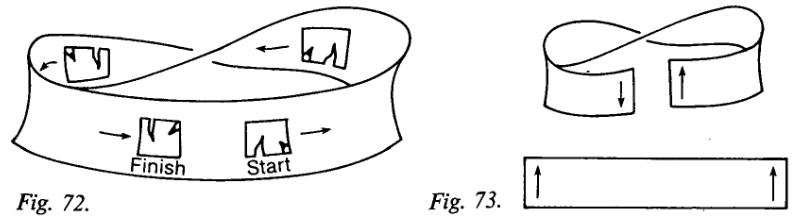
\includegraphics[scale=0.35]{./finitebutinfinite.png}
	\end{center}
	or this famous one as Klein's bottle
	\begin{center}
		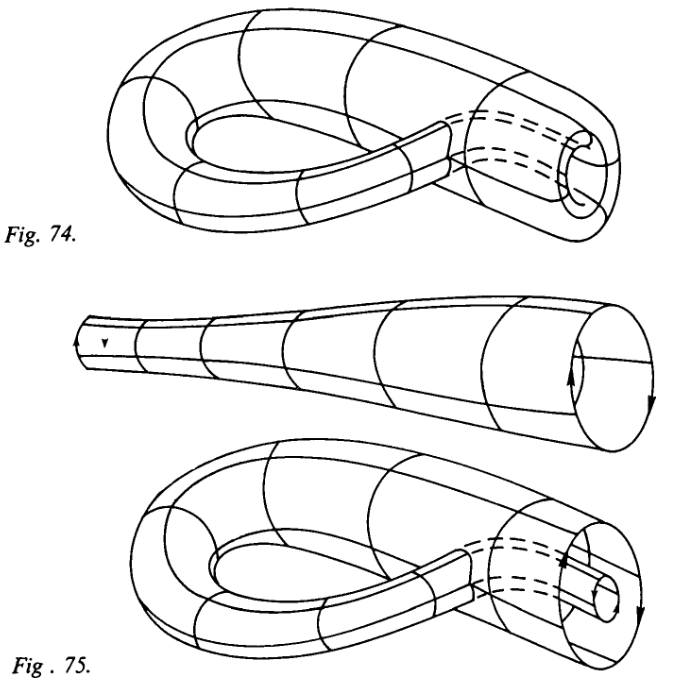
\includegraphics[scale=0.35]{./klei3d.png}
	\end{center}
	this bottle is in 3-dimention space, however, to understand its structure, we should use the definition of 4-dimention space then use the projection in two dimentional space.
	 \subsection{Riemannian Space} 
	 As mentioned above, Riemannian geometry and space has a solid connection with Einstein's Einstein's General Theory. In this part, we will walk through the history of  this geometry.
	 In the 1800s, Non-Euclidean geometry which itself does not sastify all Euclid's geometry postulates, some kinds of this gemetry class are  differential geometry, hyperbolic geometry, etc. and Riemannian geometry is one of them. 
	 In 1854, Riemann suggeted the idea of general metric. He proposed the metric be given in  a quadratic form and proportion with the derivative of square of length as 
	 \begin{center}
	 	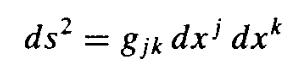
\includegraphics[scale=0.35]{./riemann_form.png}
	 \end{center}
	 the spaces which can be describled by this metric called Riemannian spaces. In his work, Riemann pointed out  the concept of curves in a two dimentional space, studied the constant curvature in multidementional spaces.
	 The metric $g_{ij}$ in Riemann space can be defined in three ways:
	 \begin{itemize}
	 	\setlength{\itemindent}{.2in}
	 	\item  Any arbitrary function in mathematics can be  made use of the metric coefficients.
	 	\item  The metric coefficients can be fittrf to exprimental data.
	 	\item  In the special cases of Euclidean space, the transformation of coordinates from Pythagorean  formular
	 	\begin{center}
	 		$ds^2 = dx^2 + dy^2 +dz^2$
	 	\end{center}
	 \end{itemize}
 	\section{Riemannian Manifolds in General Relativity}
 	A Riemannian space or a Riemannian manifold, where
 	various notions such as length, angles, areas (or
 	volumes), curvature, and divergence of vector
 	fields can be defined, is a smooth manifold with an inner product on each tangent space. 
 	Most of the properties of Riemannian space are same as in curved space.
	\subsection{Time as the Forth Dimention - The Spacetime Metric}
	\subsubsection{The Forth Dimention}
	From the previous section, we if an object is describled in three dimetional space, and we want to see how it looks like, we should place it in the higher dimention space. So, in this part we will develop a space, where 3-dimention objects trails, in four dimentions. Which aspects will be added to the current space to build  a new dimention? It depends on our purposes, it may be mathematical, spatial dimentions, or entropy, energy density, and so on.
	 
	Let imagine, we have an object whichs move from a place to anywhere else in a three dimentional space, so we need to measure how it move with information about velocities, accelerations, distances between starts and end points of motions, etc. In ur expectation , the forth dimention needs to adopt some aspects as chronological orders, mesurement of  changes, a direction, the concept of "relativity of reality", and  marking events in logical way but can not roll-back to previous physical states.  As those listed properties, we can see only one thing that make sense and familiar for us to use an abtract concept that influences all space phenomenas and events called time. For example, we take a quick look at the image below:
	\begin{center}
		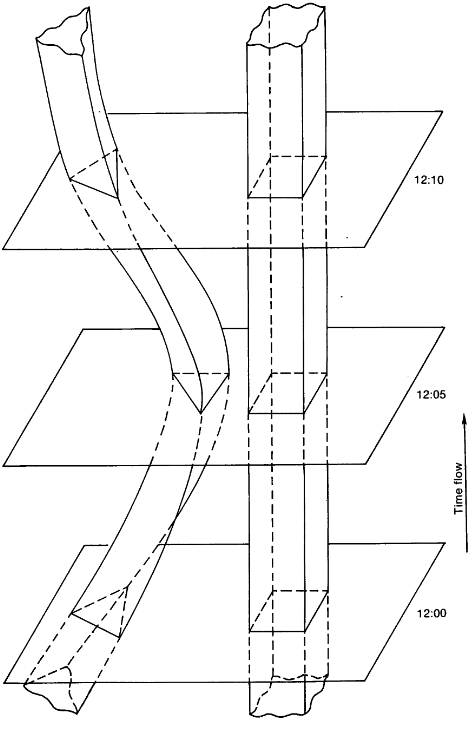
\includegraphics[angle=-90,scale=0.4]{./time_model1.png}		
	\end{center}
	In this figure,  we describe two objects as "the triangle" $\textbf{$\triangle$}$ and  "the square" $\Box$; and $\triangle$ approches to $\Box$ then slides away while $\Box$ goes straight on his way. The event is tracked  in a time direction with positive value and can not roll-back both in time and action's orders. For both $\triangle$ and $\Box$, at a specific time, they have different positions in space on each time-plan$^{\cite{minkowki}}$.  It also simulates that objects move in a plane called a time plan, in each frames of time, the objects have its own positions and can not go back in time.  Now, the question is if our space like that, why couldn't we see the past, the present, and the future at the same time? There are many reasons, however, there are two main causes that most people accept. One is that an known object must have specfic properties and can not have many diffrent states, local positions, energy at the same time. Another is if these periods of time are co-existed at the same time, we can go back to  the past - may get being younger, or move forward to predict what would be unexpectedly happend and change it but we can't.  Since this point of view,  we see that to express the state of things in logical orders we need at leat three dimentions to present objects, and one other dimention to show how the object develops - this dimention just goes on and on, and is attached to object's space.  So, space, where objects exist and trails in their  development direction, now has three dimentions and incorporates with a interval aspect - called time. This forms a new four dimentional coordinates that we call space-time. We should distinguish that space-time includes two elements as 3-dimentional space and time (as Minkowski does with his space$^{\cite{minkowki}}$); and spacetime is a single object space that an object floats in both space and time.
	\subsubsection{The Metric}
	Considering  time as a dimention in the spacetime coordination system, we can put physical events in  the system with four global coordinates $t, z, y, z$ . From the special relativity we know that laws of physics are the same in all inertial frames, so an observer in different inertial frames gets the same results for any physics phenomena with coordinate of $t', x', y', z'$. Thus, the coordinates themselves do not have any intrinsic properties because of being labling by the observers rather than the properties of spacetime itself. The spacetime has its own self-determination to clarify which qualities have pernament, independent significance observers, i.e and to reflect intrinsic structures.
	
	In  special relativity, the quantity that an observer care about is the spacetime interval, $I$, given by
	\begin{center}
		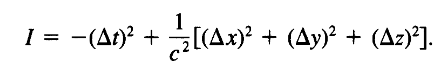
\includegraphics[scale=0.4]{./InertialFrame.png}
	\end{center}
	The interval $I$ and its function  have independent quantities from observers between events. And now we see that this interval seem to be described for ordinaty Euclidean space and should be replaced  by tensors as in the first section. 
	
	There are many theories in physics inconsistent with special relativity,  they need modification to fit  and adopt to spacetime structure. One of these theories is Newton's grativitation theory for some reasons as instantaneous interaction - lead to the confusion that information and communication travel faster than speed of light,  separation of space and time  -  observers in differrent motions have the same time and space,  consevation of mass and energy -  mass and energy does not transform to each other. However, for Einstein, there are two reasons that made him think differently and look for a new theory to create a connection between gravitation and spacetime$^{\cite{wald1984}}$.
	The first reason is that all objects are affected by gravity and themselves fall in a gravitational filed. The other is from Mach's principle. The principle states all matters in the universe have their contributions to the local distribution of other matter around them. Einstein accepted and adopted to this idea and actively, strongly motivated to look for a theory,  not like special relativity, to point out the connection of the structure of spacetime and  existence of matter.  According to these statements, the new theory which explained sucessfully the link between space, time, and gravitation was proposed - general relativity. However,  synchronously, the new theory brought out a new problem - the spacetime metric needs another form and separates from  the special relativity theory to present the physical effects of a graviational filed. Then, Einstein postulated  the spacetime is curved by  the stress-energy-monetum tensor in his famous equation
	\begin{center}
		$R_{\mu\nu} - \frac{1}{2}Rg_{\mu\nu} = 8\pi G T_{\mu\nu}
		$$^{\cite{seancarol}}$
	\end{center}
	This equation also pointed out the notion that spacetime accomplished with manifolds is a  four continous dimentional  coordinate system.
	\subsection{Gravitation as Geometry}
	As we discuss before, the spacetime is a one object which is combined both the three dimentional space where physical things in our word exist and time as the forth dimention, so it has properties of geometry when being used to describe matter located inside. However,  the gravitation field was also developed on the curved space, especially on Einstein's spacetime which was inspired by Riemannian manifolds. In this part, we try to use geometry tools to describe gravitation in the context of general relativity. We all know that gravitation is risen from the dynamical the curvature of spacetime through  tensor metric. The $\textit{Principle of Equivalence}$ helped Einstein formalize his idea to universalize the gravitational interaction. The principle presents in two main common forms. The first is the $\textit{Weak Equivalence Priciple}$ stating the inertial mass and  gravitation mass of any objectss are the same mesurement. Now, we look at several laws in physics, one is the Newton's Second Law which relates the force exerted on matter: 
	\begin{center}
		$F = m_i a$
	\end{center}	
	The object's mass (or inertial mass) has a unique value and does not depend on how strong the force is. Next, we also have Newton's law of gravitation as: 
	\begin{center}
			$F_g = - m_g \nabla\phi$		
	\end{center}
	Then the $m_g$ and $m_i$ must be equal and  $a = -\nabla \phi$. The other form of  $\textit{Principle of Equivalence}$  is $\textit{Einstein Equivalence Principle}$ shown that "In small enough regions of spacetime, the laws of physics reduce to those of special relativity,· it is impossible to detect the existence of a gravitational field by means of local experiments"$^{\cite{seancarol}}$. In some cases, there is a gap between graviational and non-gravitational laws of physics that is where Strong  Equivalence Principle will be defined  to consist all off  physics' laws.
	
	According with these experiments to  prove the equality of innertial and gravitational mass, we need tools to show how is it correct in both theoretical and mathematical ways.  From the universal phenomena as Doppler effect, gravitational redshift, we need to consider laws in a tiny space which is enough to consider our spacetime as a flat plan. The new methods given based on  the idea of gravity as a force spreading through spacetime is to imagine spacetime has a curved geometry, and gravitaion  is here in the form of this curvature. the mathematical structure and method should be used is  a differentiable manifold. 
	\subsection{Riemannian Manifolds (Space)}
	In this section, we will study Riemannian manifolds and its application in the Einstein's General Relativity theory.
	\subsubsection{Type of Manifolds}
	In physics, we use both two kinds of Riemannian manifolds to express the physical world,  Riemannian manifolds and semi (pseudo) - Riemnannian manifold. The different between them is that semi-Riemannian manifolds accepts all both positive and negative values in its metric tensor while the last one only takes positive values.  Although both kinds of Riemannian manifolds have the same common properties, they have different applications. For the Riemannian manifold they use in differential geometry, topology, and optimization; while the other is used in a study of spacetime in general relativity, mathematical physics to deal with spacetime curvature, gravitational fields, and the causal structure of spacetime because of its developed tools by mathemticians. And in Riemannian manifolds, the metric tensor is considered as inertial-gravitational potential.
	\subsubsection{General Structure }
	As mentioned in the first section, the distance ds between two separated points is a quadratic form:
	\begin{center}
		$ds^2 = g_{ij} (x)dx^i dx_J$
	\end{center}
	in a small and limited local plane of a curved space we can consider the curved plane as a flat plan, so  geometry looks like in the Euclidean space or space-time in cases of relativity.  If there is no specific coordinate systemt indicated, the transformation of this formular is extended to all posible coordinate differences and has a gemetrical properties of space (also time if the space and time is as a single object), then  $ds^2$ is independent of the used coordinates. In oder to satisfy space metric tensor elements must change in a way under coordinate changes. So, $x^{i'} = x^{i'}(x^i)$ , then  $dx^i = \frac{\partial x^i}{\partial x^{i'}} dx^{i'}$, and we have
	\begin{center}
		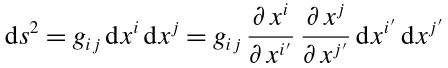
\includegraphics[scale=0.4,alt={coordinate change}]{./rie_chang_1.png}
	\end{center}
	Due to changes in the object location, and we want the distance interval  $ds$ have the same value when comapring to the old coordinate system,  the metric tensor components in the new system must be
	\begin{center}
		$g_{i'j'} = g_{ij} \frac{\partial x^i}{\partial x^{i'}} \frac{\partial x^j}{\partial x^{j'}} $
	\end{center}
	Now, we determine the coefficients for tensor transformation 
	\begin{center}
		$\Lambda^{j}_{j'} = \frac{\partial x^J}{\partial x_{j'}}$
	\end{center}
	and the transformation of  a contravariant vector as
	\begin{center}
		$V^{j'} = \frac{\partial x^{j'}}{\partial x_{j}} V^j$
	\end{center}
	then, we turn $x^i $ to a function of $\tau$ as $x^i = x^i (\tau)$, and replace to $V^i$ above with $V^i = \frac{ds^i(\tau)}{d\tau}$, so 
	\begin{center}
		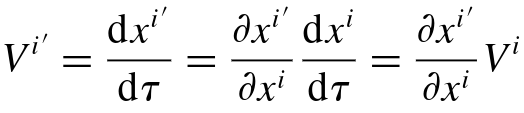
\includegraphics[scale=0.2]{./Vi_diff.png}
	\end{center}
	An invariant function O which behaves as a component of covariant vector should have derivatives
	\begin{center}
		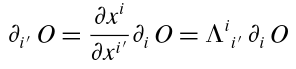
\includegraphics[scale=0.35]{./deriva_O_teno.png}
	\end{center}
	If the second term equals to zero or to be vanished, the coordinates turns in to the linear one. The derivatives act on both covariant vector component and tensor components, however, this does not make a tranformation on the components of a covariant vector.
	\begin{center}
		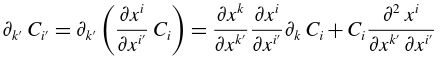
\includegraphics[scale=0.5]{./driva_cova_vec.png}
	\end{center}
	In this case, the tensor character - the last one term -  result to be symetric, and the partial derivative  $\partial_k C_i - \partial _i C_k$ does not have tensor character so it is antisymmetry.
	\subsubsection{Torsion tensor}
	The commutator of the covariant  derivative acting on  a scalar $\Phi$ is called  the torsion tensor $S^{\mu}_{\kappa \lambda}$ 
	\begin{center}
		$[D_{\kappa}, D_{\lambda}] \Phi = S^{\mu}_{\kappa \lambda} \pdv{\Phi}{x^{\mu}}$
	\end{center}
	and $S^{\mu}_{\kappa \lambda}$ can be expressed as
	\begin{center}
		\fbox{$S^{\mu}_{\kappa \lambda} = \Gamma^{\mu}_{\kappa \lambda} - \Gamma^{\mu}_{\lambda \kappa}$}
	\end{center}
	and we have $D_{\lambda} \Phi = \pdv{\Phi}{x^{\lambda}}$
	\subsubsection{Geodesics}
	In mathematics, geodesics is curves thoes parallel-transports their own tangent vectors. It means in physics, the motion $f$ which is describled as a function can have geodesic shape when having its second derivative as zero$^{\cite{geo_Schutz}}$.
	\begin{center}
		$f'' = 0$
	\end{center}
	If $\lambda$ is a curve parmeter, and we places ${x^i}$ is as any coordinates of  space system, the geodesic has form of
	\begin{center}
		$\dv{f^i}{\lambda} + \Gamma^i_{jk} f^i f_k = 0$
	\end{center}
	the $\Gamma^i_{jk} $ is a Christoffel symbol which will be introduced in the next section.
	\subsubsection{Christoffel Symbols}
	Fundamentally, in differential geometry and general relativity, to discribe how vectors change in tengent spaces of nearby points and under parallel transport along a curved surface, we use a symbol with relating to the metric  and reflecting changes of vectors in an object called the \textit{Christoffel symbol}
	\begin{center}
		$\Gamma^{\lambda}_{\mu \nu} = \dfrac{1}{2} g^{\lambda \sigma} (\partial_{\mu}{g_{\nu \sigma}} + \partial_{\nu}{g_{\sigma \mu}}- \partial_{\sigma}{g_{\mu \nu}})$
	\end{center}
	then,  genralizing the partial derivative, the covariant derivative  of a vector field is transfromed as 
	\begin{center}
		$\nabla_{\mu} V^{\nu} = \partial_{\mu} V^{\nu} + \Gamma^{\nu}_{\mu \sigma} V^{\sigma}$
	\end{center} 
	after that, the geodesic equation in form of
	\begin{center}
		$\dv[2]{x^{\mu}}{\lambda} + \Gamma^{\mu}_{\rho \sigma} \dv{x^{\rho}}{\lambda} \dv{x^{\sigma}}{\lambda} = 0$
	\end{center}
	is also considered as metric coefficients. And, now, we put $f^{\rho} \equiv \dv{x^{\rho}}{\lambda}$ and $f_{\sigma} \equiv \dv{x^{\sigma}}{\lambda}$, the previous form of the geodesic equation appears.	
	\subsubsection{Ricci Tensors}
	The Ricci tensor is defined by
	\begin{center}
		\fbox{$R_{\alpha \beta} :=  R^{\mu}_{\alpha \mu \beta}  = R_{\beta \alpha}$}
	\end{center}
	and on that result, we can see  Ricci scalar as
	\begin{center}
		\fbox{$R := g^{\mu \nu} R_{\mu \nu}  = g^{\mu \nu} g^{\alpha \beta} R_{\alpha \mu \beta \nu}$}
	\end{center}
	\subsubsection{Einstein Tensors}
	The Einstein's tensor $G_{\kappa \mu}$
	\begin{center}
		\fbox{$G_{\kappa \mu} \equiv  R_{\kappa \mu} - \dfrac{1}{2} g_{\kappa \mu} R$}
	\end{center}
	When applying Ricci and metric tendors to torsion, we get that Einstein's tensor have symetry as
	\begin{center}
		$G_{\kappa \mu} = G_{\mu \kappa}$
	\end{center} 
	and this have upto 10 independent  components.
	\subsubsection{Others}	
	In this section, we will walk through some orthers tools or definitions which was developed in maninfolds or especially in (semi/peusdo) Riemannian manifolds
	\begin{itemize}
		\item From Jacobi indentities:
		\begin{center}
			$[D_{\kappa}[D_{\lambda},D_{\mu}]] + D_{\lambda}[D_{\mu},D_{\kappa}]] + D_{\mu}[D_{\kappa},D_{\lambda}]] $
		\end{center}
		we can take the Bianchi identities with vanishing torsion parts
		\begin{center}
			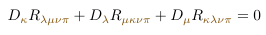
\includegraphics[scale=0.5]{./bianchi_sl.png}
		\end{center}
		and the torsion-free Bianchi identities could be written as 
		\begin{center}
			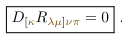
\includegraphics[scale=0.5]{./tor_fre_bian.png}
		\end{center}
		\item Coordinate 4-velocity \\
		With a partical which is moving along a line 
		\begin{center}
			$x^{\mu}(\tau)$
		\end{center}
		and $\tau$  is the time of a particle. The proper time is defined  by $d \tau \equiv \sqrt{-ds^2}$, then the coordinate 4-velocity $u^{\mu}$
		\begin{center}
			\fbox{$u^{\mu} \equiv \dv{x^{\mu}}{\tau}$}
		\end{center}
		the square of  4-velocity value is contant
		\begin{center}
			\fbox{$u_{\mu}u^{\mu} = g_{\mu \nu} \dv{x^{\mu}}{\tau} \dv{x^{\nu}}{\tau} = \dv{s^2}{{\tau}^2} = -1$}
		\end{center}
		\item  Coordinate 4-momentum
		As a result, we now have the coordinate 4-momentum  of a particle  of rest mass  $\textit{m}$ is
		\begin{center}
			\fbox{$p^{\mu} \equiv mu^{\mu} = m \dv{x^{\mu}}{\tau}$}
		\end{center} 
		from the above,  the square of momentum is 
		\begin{center}
			$p_{\mu} p^{\mu} = m^2 u_{\mu} u^{\mu} = - m^2$
		\end{center}
	\end{itemize}
	\subsection{Application in General Relative}
	For  this last section of this par, we will walk throught some application of curved space - especially Riemannian and Semi Riemannian Manifold in physics.
	\subsubsection{A Part that Helps to Form General Relativity}
	Base on Einstein lecture and in his paper, he agreed that he used manifolds and other approaches to form his famous one theory and space that, now, we call Einstein's spacetime.
	\subsubsection{Approximated to Special Relative} 
	In some previous section, we should know that the manifolds can be view as a flat plane in a small enough space - locality. Then we revisit this using approximated method. 
	The approximate should be raise as an event p in spacetime M, then the speciall relative exist in the tangent space $T_{p}(M) \approx R^4_1$, and  an exponetial map $e_p$ provides a method of comparision between them. Take a look in local flatness region, a small neighborh, the $T_{p}(M)$  is an approximation from the General Relativity to the Special Relativity. When the data of recorded event meets Newtonian limitation  
	\begin{center}
		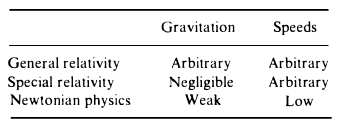
\includegraphics[scale=0.5]{./neton_limit.png}
	\end{center}
	the General Relativity tend to  Newtonian result.
	\subsubsection{Matter Curves Spacetime}
	We also know that free fall objects are afected by gravity. In Newtonian physics, we place this motion into two categories as accelerating and non-accelerating without considering whether object can cause back an other effect on space. Einstein did not agree with this assumtion, he thought that all free fall is geodesic in spacetime; the gravitation of an object is not bend any connection line in space but to bend the spacetime which is describle having geodesics.
	\subsubsection{The Schwarzschild Solution}
	In the Schwarzschild space - which was developed on semi Riemannian Manifolds , it indicates a singularity point that appear at $r = 0$ when
	\begin{center}
		$R^{\mu \nu \rho \sigma} R_{\mu \nu \rho \sigma} = \dfrac{48 G^2 M^2}{r^6}$
	\end{center}
	However, there is a hard question at $r = 2GM_{\odot}$, what will happend there? 
	From the Schwarzschild solution, we have the stable circular orbit must larger than $6GM$,  and in range of $3GM$ and $6GM$, it is unstable; then under $3GM$, matter accelerates continuously and nothing can stop it - at $r = 2GM$ either. As a result of this solution, it also states that the existence of black holes in physical world. 
	\subsubsection{The Existence of Black Holes}
	As mentioned above, in this section we will explore Schwarzschild black holes. Apply the space-time metric of Minkowki, we could see that the light cone of this space-time model will be close when $r = 2GM$, and the derivative of  $\dv{s}{t} \rightarrow \infty$, and below is the figure to illustrate how it is
	\begin{center}
		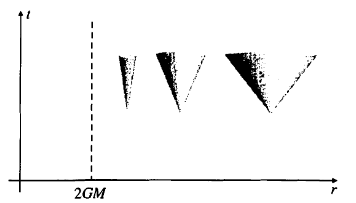
\includegraphics[scale=0.5]{./con_close.png}
	\end{center}
	after closing up, in the tortoise model and coordinate, we could expect matter will be pulled out in, however, it will be remain their for later discussion as well as the extension and more application of the Schwarzschild solution.
	\subsubsection{General Relativity as A Geometric Presentation}
	Through the beginning, we all treat space, space-time (as Minkowkian space), or spacetime (as Einstein does with 4-dimentional space in the union of 3-dimentional space and time as a single object) in a graph or figure to visuallize what they are, and trully, in physical world, our space is also. In the spacetime presentation of General Relativity, we contruct some new definitions
	If ($M^n$, g) is a spacetime, a vector $X_p \in T_p M_n$ is called \\
	\begin{enumerate}
		\item spacelike if $g(X_p, X_p) > 0$
		\item timelike if $g(X_p, X_p) < 0$
		\item lightlike if $g(X_p, X_p) = 0$ but $X_p = 0$
		\item causal if it is timelike or lightlike. 
		\item causal curves are those piecewise smooth curves which are piecewise timelike or lightlike
		indifferently. 
	\end{enumerate}
	
	and on these definition, we have some things disscussed above as mathematical assumtion, equivalent priciples, approximation to transform from General Relativity to Newtonian mechanics and laws, Fermi-Walker’s transport in Lorentzian manifolds.
	\section{Comparison with Other Mathematical Frameworks}
	To explain how Riemannian Manifolds benefits us in studying structure of spacetime and other area in physics, we will  take a short  course to clarify the disavantages of some mathematical spaces:
	\subsection{Calibration Hyperbola}
	\begin{center}
		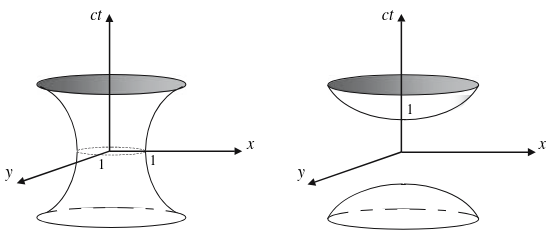
\includegraphics[scale=0.5]{./hyper_space.png}
	\end{center}
	This mathematical space is considered as two reference systems are represented in a same coordinate system and in the same diagram, the scales of their axes are different and require calibration. It looks good to present a spacetime structure, however, this struggles in to some several problem.
	As in the figure, we can see there are two types of this model, so this requires a large effort for calibration and may be a huge challenge. Futhermore, hyperbolic spaces also require a lot of intricate form and have unexpected abtract mathematical contructions while Riemannian manifolds are easy to define any subspaces.
	\subsection{Light Cone}
	There are several space-time structure cunstructed with the idea of light cones, however, it's not there. In this case, we only pay attention to a light cone model.
	\begin{center}
		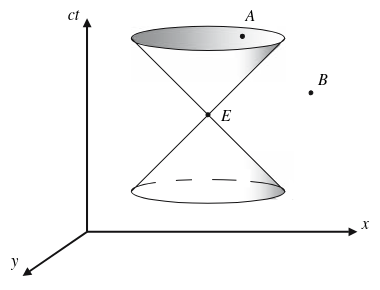
\includegraphics[scale=0.5]{./lih_cone.png}
	\end{center} 
	This model have some disadvantage to describle space time as the event which happend in this model must be defined itself as a space-like, time-like, or light-like. The step of this consideration in some cases may be hard and can not be done.  In addtion, when using line cone, we can not describle some aspect of spacetime like sparial, cuvers on surface, and it does not have developed transformation method to switching between general and special relative.
	\subsection{Timelike Separated Events} 
	In general, the timelike sparated event is a model which inherites  from a light cone model. However, this imply the fundamental of understading causality and propagation of physicall actions and interacions in relativity. The disadvantage of this model is that it can not present spacetime curvature as well as an effect of massive objects on the system.
	\begin{center}
		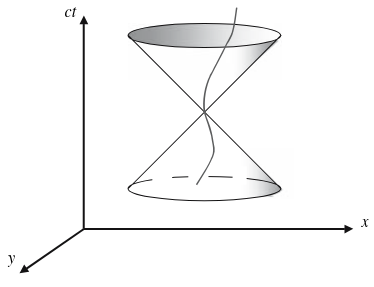
\includegraphics[scale=0.5]{./lih_cone_time.png}
	\end{center}
	\section{Applications Beyond General Relativity}
	Beside the application in the General Relativity, Riemannian and semi-Riemannian manifolds also have contributed to other theory in physics such as the Hawking singularity theorem, the Penrose singularity theorem, homogeneous and isotropic in cosmology. Moreover, Riemnian manifolds also play an crucial role in String theory when mentioning and studying  string propagation,  contraints, compactification field.
	\section{Conclusion}
	After taking the course of general relativity, we could see that, in our current physics, we are using mixed methods and spaces (curved spaces, flat plane space, or a combination of both flat-plane and curved space) to describle our world as well as transfering and transforming from one to other spaces or coordinate systems.
	\section{Refferences}
	\begin{thebibliography}{9}
		\setlength{\itemindent}{.2in}
		\bibitem{wald1984}
		Robert Wald, \emph{General Relativity}, University of Chicago Press (June 15, 1984).
		\bibitem{RudolfBVRucker}
		Rudolf V B Rucker, \emph{Geometry, Relativity and the Fourth Dimension}, Dover Publications, Inc. (1977)
		\bibitem{minkowki}
		Hermann Minkowski, \emph{Space and Time Minkowski’s Papers on Relativity}, Minkowski Institute Press (2012)
		\bibitem{benjaminzhou}
		Benjamin Zhou, \emph{Lecture note on Spacetime Geometries}, Stanford University (2016)
		\bibitem{seancarol}
		Sean Carol, \emph{Spacetime and Geometry: An Introduction to General Relativity}, PEARSON Press (2014)
		\bibitem{rafael}
		Rafael Ferraro, \emph{Einstein's space-time: An Introduction to Special and General Relativity }, Springer (2007)
		\bibitem{geo_Schutz}
		Bernard F. Schutz, \emph{Geometrical Methods of Mathematical Physics}, Cambridge University Press; (1980)
		\bibitem{gra_Misner}
		Charles W. Misner, Kip Thorne, John Archibald Wheeler, \emph{Gravitation}, Princeton University Press (2017)
		\bibitem{einGen_Oy}
		Øyvind Grøn and Sigbjørn Hervik, \emph{Einstein's General Theory of Relative}, Springer (2007)
		\bibitem{halmiton_GR}
		Andrew J. S. Hamilton, \emph{General Relativity, Black Holes, and Cosmology}, Cambridge University (2020)
		\bibitem{semiRie}
		Newman, Stephen C., \emph{Semi-Riemannian geometry - the mathematical language of general relativity}, Wiley (2019)
		\bibitem{valter_geo}
		Valter Moretti, \emph{Geometric Methods in Mathematical Physics II Tensor Analysis on Manifolds and General Relativity}, Department of Mathematics, University of Trento, Italy
		\bibitem{GR_Schutz}
		Bernard F. Schutz, \emph{A First Course in General Relativity - Second Edition}, Cambridge University Press; (2009)
		
	\end{thebibliography}
\end{document}